%MIT OpenCourseWare: https://ocw.mit.edu
%RES.18-011 Algebra I Student Notes, Fall 2021
%License: Creative Commons BY-NC-SA 
%For information about citing these materials or our Terms of Use, visit: https://ocw.mit.edu/terms.

\section{The Projection Formula}
\subsection{Review: Symmetric and Hermitian Forms}
Last time, we were talking about different kinds of pairings or bilinear forms on vector spaces. In particular, we will be studying two cases in parallel: vector spaces $V$ over $\RR$ with symmetric forms on them, and vector spaces over $\CC$, with Hermitian forms on them. A Hermitian form is almost symmetric, with a complex conjugate thrown in.

Then, we discussed the idea of vectors being \emph{orthogonal} to each other with respect to the form if the pairing is zero. A form is non-degenerate if and only if the space of vectors orthogonal to the entire vector space $V$ is $\{0\},$ so there are no nonzero vectors orthogonal to all other vectors. Such a vector lies in the kernel of the matrix of the form, so a matrix with nonzero determinant will correspond to a non-degenerate form. 


\subsection{Orthogonality}

Recall this theorem about the restriction of a bilinear form to a subspace. We'll prove it now.
\begin{theorem}\label{non-degenerate stuff}
Let $W \subseteq V.$ If $\bform|_W$ is non-degenerate on $W,$ then $V = W \oplus W^{\perp}$, which means that every vector $v \in V$ is equal to $\vv{w} + \vv{u}$ uniquely, where $w \in W, u \in W^\perp$. 
\end{theorem}

It is possible for the restriction of a non-degenerate form to be degenerate; for example the form $A = \begin{pmatrix}0 & 1 \\ 1 & 0\end{pmatrix}$ is non-degenerate but is just given by $A' = 0$ when $W = \text{Span}(\vec{e}_1),$ which is clearly degenerate.

\begin{proof}
If $\bform|_W$ is non-degenerate, then $W \cap W^\perp = \{0\}.$ We have $W \oplus W^\perp \subset V,$
so it suffices to show that $V \subset W \oplus W^\perp.$ Pick a basis of $W,$ $\{w_1, \ldots, w_k\},$ and define a linear transformation 
\begin{align*}
    \varphi: V &\rto \CC^k \\
    \vec{v} &\mto (\langle w_1, v, \rangle, \ldots, \langle w_k, v \rangle).
\end{align*}
This is a linear transformation just by the properties of a Hermitian form.
The kernel is \[
\ker(\varphi) = W^\perp,
\]
since $W = \text{Span}\{\vec{w_i}\}.$ Also, $\dim \im \varphi \leq k = \dim W,$ so by the dimension formula,
\[
\dim V = \dim \ker\varphi + \dim \im \varphi \leq \dim W^\perp + \dim W.
\]

Consider the mapping
\begin{align*}
    W \oplus W^\perp &\rto V \\
    (w, u) &\mto w + u.
\end{align*}
It has kernel $\{0\},$ since $W \cap W^\perp = \{0\},$ so 
\[
\dim W + \dim W^\perp \leq \dim V,
\]
and thus $\dim W + \dim W^\perp = \dim V$ and therefore $V = W \oplus W^\perp.$
\end{proof}

To emphasize, the geometric version of this with respect to the dot product feels obvious and works in most cases. For general forms, we have to have this condition that our form is non-degenerate on the subspace.

The splitting $V = W \oplus W^\perp$ is helpful, in particular, for inductive arguments, because it is possible to reduce some property of $V$ to being true on $W$ and $W^\perp.$

\subsection{Orthogonal Bases}

By applying a change of basis, it is always possible to put an arbitrary matrix into Jordan normal form, and if there are distinct eigenvalues, it is in fact possible to diagonalize it. What about the matrix of a bilinear form?
\begin{qq}
Given a vector space $V$ and a bilinear form $\bform,$ how simple can we get the form to be?
\end{qq}

First, it is always possible to find a basis orthogonal with respect to the bilinear form. 

\begin{theorem}
For a symmetric or Hermitian form $\bform,$ the vector space $V$ has an orthogonal basis $\{v_1, \cdots, v_n\}$, which is when $\langle v_i, v_j \rangle = 0$ for $i \neq j.$ The matrix for the pairing in the basis will then be diagonal, since it is given by the inner product from the form. 
\end{theorem}

\begin{proof}
To prove this, induct on $\dim V = n.$ 
\begin{itemize}
    \item \textbf{Case 1.} There is some $u$ such that $\langle u, u \rangle \neq 0.$ Then, the one-dimensional subspace $W = \text{Span}(u),$ $\bform|_W$ is non-degenerate. 
    
    By induction, $W^\perp$ has an orthogonal basis $\{v_2, \cdots, v_n\}$, so $\{u, v_2, \cdots, v_n\}$ is an orthogonal basis for $V.$
    
    \begin{center}
    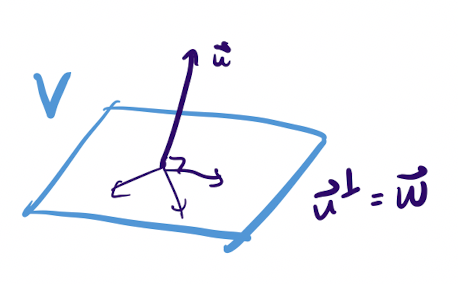
\includegraphics[width=5cm]{Lecture Files and Images/lec26-thm.png}
\end{center}

    \item \textbf{Case 2.} Otherwise, for every $v \in V,$ $\langle v, v \rangle = 0.$ This is a very strong constraint on the form, and in fact it forces $\langle v, w\rangle = 0$ for all $v, w,$ which forces \emph{any} basis to be an orthogonal basis. 
    To see this, consider the inner product on a sum of two vectors with itself:
    \begin{align*}
        0 &= \langle v + w, v + w \rangle \\
        &= \langle v, v \rangle + \langle w, w \rangle + \langle v, w \rangle + \langle w, v\rangle \\
        &= 2\langle v, w \rangle.
    \end{align*}
    When $F = \RR,$ we have $\langle v, w \rangle = 0,$ by the symmetry of the form. Otherwise, for $F = \CC,$ $\text{Re}(\langle v, w \rangle) = 0,$ and the same process can also be done for $v$ and $iw$ to show that $\langle v, w \rangle = 0.$ Then the inner product is 0 on any two vectors so every basis is orthogonal.
    %include this argument for \CC
\end{itemize}
\end{proof}
We can simplify the basis even further.
\begin{corollary}
In fact, $V$ has an orthogonal basis $\{v_1, \cdots, v_k\}$ where $\langle v_i, v_i\rangle = 1, -1,$ or 0. 
\end{corollary}
\begin{proof}
Take an orthogonal basis $\{x_1, \cdots, x_k\}$. Consider $\langle x_i, x_i \rangle$, which is a real number.
\begin{itemize}
    \item If the pairing is 0, then let $v_i = x_i.$
    \item Otherwise, we can normalize and take $v_i = \frac{1}{\sqrt{|\langle x_i, x_i \rangle|}}x_i;$ then $\langle v_i, v_i \rangle = \frac{\langle x_i, x_i \rangle}{|\langle x_i, x_i \rangle|},$ so it will be 1 or -1 depending on the sign of $\langle x_i, x_i \rangle.$
\end{itemize}
\end{proof}

In particular, if $\bform$ is non-degenerate, only $\pm 1$ occur. Also, if $\bform$ is positive definite, by definition, $\langle v, v \rangle > 0$ if $v \neq 0,$ so only $+1$s occur, so in that basis, the form looks just like the dot product or the standard Hermitian product.

The following claim will be shown in the upcoming problem set.

\begin{claim}[Sylvester's Law]
In fact, given $V$ and $\bform,$ the number of 1s, the number of -1s, and the number of 0s that occur in the diagonal form are determined by $V$ and $\bform,$ and not by the choice of orthogonal basis.\footnote{They are similar to eigenvalues in that while there are many choices of orthogonal basis, the \emph{number} of 1s, -1s, and 0s are not dependent on the particular basis.} This is called \emph{Sylvester's Law}, and the number of 1s, -1s, and 0s is called the \emph{signature} of the form. 
\end{claim}

For example, in the form used in special relativity, $\begin{pmatrix}-1 & & & \\ & 1 & & \\ & & 1 & \\ & & & 1\end{pmatrix}$, the signature is $(3, 1, 0).$

 %what does he say here LOL i missed it (below)
In matrix form, the corollary states that for a symmetric matrix $A \in \text{Mat}_{n \by n}(\RR)$, for which $A^T = A,$ there exists some matrix $P \in GL_n(\RR)$ such that $P^TAP$ is a diagonal matrix with all $1s, -1s$, or 0s on the diagonal:
\[
P^TAP = \begin{pmatrix} 1 & & & & & \\ & \ddots & & & &  \\ & & -1 & & &  \\ & & & \ddots & & \\ & & & & 0 & \\ & & & & & \ddots \end{pmatrix}.
\]

If $A$ is positive definite, which is when $x^T Ax > 0,$ there exists $P$ such that $P^TAP = I_n$ implies that $A = Q^TQ$, where $Q= P^{-1}$.

The statement is similar for complex matrices, where we replace the transposes with adjoints.
%add the statement for complex matrices
%ethany: i feel like this is unnecessary

%is the number of 1s and -1s set? ok sylvester's whatever

%what is the importance of the signature? does it tell you anything about the metric given by the inner product? 

\subsection{Projection Formula}

Consider a vector space $V$ and a form $\bform$, as well as a subspace $W$ for which $\bform|_W$ is non-degenerate. By Theorem \ref{non-degenerate stuff}, $V = W \oplus W^\perp$ such that $v = w + u.$ 

\begin{center}
    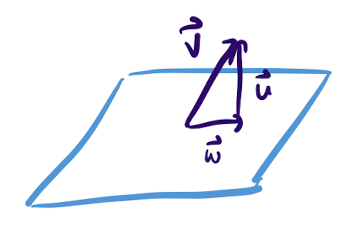
\includegraphics[width=5cm]{Lecture Files and Images/lec26-projection.png}
\end{center}

\begin{qq}
How can we compute $w$ and $u$?
\end{qq}
To do so, we use the orthogonal projection. We want a map
\begin{align*}
    \pi: V &\rto W \\
    v &\mto w,
\end{align*}
so that $v = \pi(v) \perp W.$\footnote{This is an extremely useful application of linear algebra! In geometric situations, the vector $w$ is the vector closest to $v$ of the vector in the plane, and perhaps these vectors are in a vector space of data points. Finding a formula for $w$ explicitly is called least-squares regression.}

Assuming there exists an orthogonal basis $\{w_1, \cdots, w_k\}$ for $W$, the formula for $\pi$ is simple.\footnote{Once we've developed the machinery for bilinear forms, these ideas become a lot simpler!} The vector can be written as 
\[
v = cw_1 + \cdots + cw_k + u,
\]
where $u \perp W.$ Then for all $i$, 
\[
\langle w_i, v \rangle = 0 + \cdots + 0 +c_i \langle w_i, w_i \rangle + 0 + \cdots + 0,
\]
so 
\[
c_i = \frac{\langle w_i, v\rangle}{\langle w_i, w_i \rangle}.
\]
It is not possible for $\langle w_i, w_i\rangle = 0,$ because the form would be degenerate. In fact, this formula is useful when $W = V$, because it provides a formula for the coordinates of some vector with respect to the orthogonal basis. 

\begin{example}
Let $V = \RR^3$ and $\bform$ be the dot product. Then let $W$ be the span of $\vec{w}_1 = (1, 1, 1)^T$ and $\vec{w}_1 = (1, 1, -2)^T.$ The pairings are $\langle w_1, w_1 \rangle = 3,$ $\langle w_2, w_2 \rangle = 6,$ $\langle w_1, v \rangle = 6,$ and $\langle w_2, v \rangle = -3.$ The projection of $(1, 2, 3)$ is then 
\[
\pi(v) = \frac{6}{3}w_1 -\frac{1}{2}w_2 = \begin{pmatrix}3/2 \\ 3/2 \\ 3\end{pmatrix}.
\]

To verify, $v - \pi(v) = (-1/2, 1/2, 0),$ which is orthogonal both to $w_1$ and $w_2.$
\end{example}

\newpage